%-------------------------------------------------------------
\subsection{Example 1} \label{sec:ch5:example1}

%-------------------------------------------------------------
\subsubsection{Description}

For the first example, we will consider the problem on pp.~166--167 from Ref.~\cite{Bryson1975a}:%
\begin{subequations}%
\begin{align}
\min_{u(t)} \quad & \frac{1}{2}\int_0^{t_f} u^2 dt \\
\text{subject to:} \quad & \dot{\bm{\xi}} = \begin{bmatrix} 0 & 1 \\ -1 & 0 \end{bmatrix} \bm{\xi} + \begin{bmatrix} 0 \\ 1 \end{bmatrix} u \\
& {\xi}_1(0) = x_0, \quad {\xi}_2(0) = v_0, \quad {\xi}_1(t_f) = 0, \quad {\xi}_2(t_f) = 0
\end{align} 
\end{subequations}%

\noindent Although there are no path constraints, both the initial and final state values are fully constrained. 
As a result, this problem does not fit many traditional \lqdo{} problem definitions such as Prob.~(\ref{eq:ch5:lqr}).
The structure-based problem description for this example is:%
\allowdisplaybreaks[1]%
\begin{subequations}%
\begin{gather}
% Lagrange term
\mathcal{L}\xind{1}.\xvar{left} = 1, \quad \mathcal{L}\xind{1}.\xvar{right} = 1, \quad \mathcal{L}\xind{1}.\xvar{matrix} = 1/2 \\
% system dynamics
\bm{A} = \begin{bmatrix} 0 & 1 \\ -1 & 0 \end{bmatrix}, \quad \bm{B} = \begin{bmatrix} 0 \\ 1 \end{bmatrix} \\
% linear equality constraints
\mathcal{LB}\xind{1}.\xvar{right} = 4, \quad \mathcal{LB}\xind{1}.\xvar{matrix} = \begin{bmatrix} x_0 & v_0 \end{bmatrix}\tran \\
\mathcal{LB}\xind{2}.\xvar{right} = 5, \quad \mathcal{LB}\xind{2}.\xvar{matrix} = \begin{bmatrix} 0 & 0 \end{bmatrix}\tran \\
\mathcal{UB}\xind{1}.\xvar{right} = 4, \quad \mathcal{UB}\xind{1}.\xvar{matrix} = \begin{bmatrix} x_0 & v_0 \end{bmatrix}\tran \\
\mathcal{UB}\xind{2}.\xvar{right} = 5, \quad \mathcal{UB}\xind{2}.\xvar{matrix} = \begin{bmatrix} 0 & 0 \end{bmatrix}\tran
\end{gather} 
\end{subequations}%
\allowdisplaybreaks[0]

\noindent The \textsc{Matlab} code is in Sec.~\ref{sec:ex1-code}.

%-------------------------------------------------------------
\subsubsection{Solution}

\begin{figure}
\centering

\begin{subfigure}{0.5\textwidth}
\centering
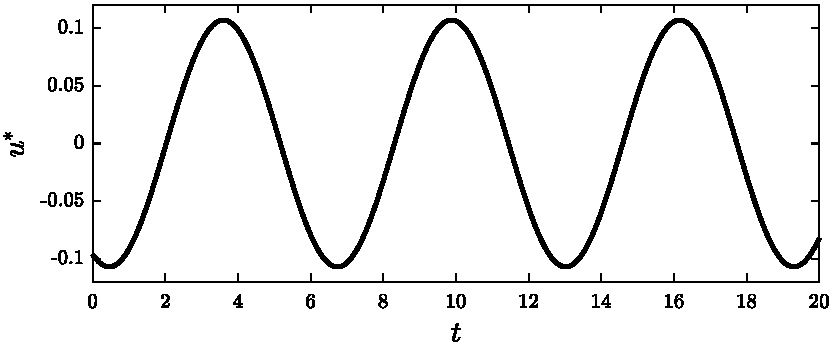
\includegraphics[width=\textwidth]{../ch5/figures/ex1sol-controls}%
\caption{Control.}
\label{fig:ch5:ex1sol:controls}
\end{subfigure}%
\begin{subfigure}{0.5\textwidth}
\centering
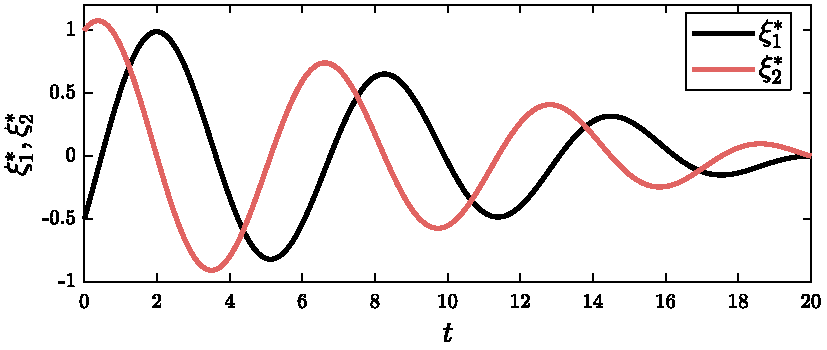
\includegraphics[width=\textwidth]{../ch5/figures/ex1sol-states}%
\caption{States.}
\label{fig:ch5:ex1sol:states}
\end{subfigure}%

\caption{Solution for \nameref{sec:ch5:example1}.}
\label{fig:ch5:ex1sol}
\end{figure}

It can be shown that the control trajectory that minimizes the objective while satisfying the constraints is:
\begin{align}
u^{\glsfoo[noindex]{optimal}}(t) = -\frac{2}{t_f^2 - \sin^2(t_f)}
\begin{bmatrix}
x_0 \\ v_0 
\end{bmatrix}\tran
\begin{bmatrix}
\sin(t_f -t) \sin(t_f) - t_f \sin(t) \\
-\cos(t_f -t) \sin(t_f) + t_f \cos(t)
\end{bmatrix}
\end{align}

\noindent with an optimal objective function value of:
\begin{align}
\Psi^* = \frac{t_f \left({v_{0}}^2+{x_{0}}^2\right)+2 {t_f}^2 v_{0} x_{0}-\cos\left(t_f\right) \sin\left(t_f\right) \left({v_{0}}^2-{x_{0}}^2\right)}{{{t_f}^2 - \sin\left(t_f\right)}^2} -2 v_{0} x_{0}
\end{align}

\noindent The problem parameters used are $t \in [0, 20]$, $x_0 = -1/2$, and $v_0 = 1$.
With these parameter values, $\Psi^* = 0.059842$.
The optimal trajectories for both the control and states is shown in Fig.~\ref{fig:ch5:ex1sol}.

%-------------------------------------------------------------
\subsubsection{Numerical Results}

% (convergence)
The convergence results for the eight tested schemes are shown in Fig.~\ref{fig:ch5:ex1sens:objective} (objective) and Fig.~\ref{fig:ch5:ex1sens:control} (controls).
The best scheme in terms of overall convergence rate was LGL-PS-G (7), and it is nearly linear.
However, once the scheme's accuracy was near machine epsilon, an accuracy threshold was reached and even started to slowly diverge (perhaps due to small errors in the calculation of the differentiation matrix, weights, etc.).
The next best scheme was CGL-PS-CC (8). 
It seemed to have a similar convergence rate as the other PS-based scheme, but it eventually achieves a sublinear rate of convergence until it reaches the precision threshold (for the objective value).

The SS-based schemes now remain. The best was ED-HS-CQHS (5), although ED-RK4-CQHS (6) was only slightly worse.
These are the two schemes that utilize the proposed CQHS quadrature method.
The convergence rate seemed to be sublinear, and an objective value accuracy threshold was reached for both schemes.
The control error between these schemes was nearly identical.
Next, perhaps surprisingly, was ED-ZOH-CEF (1).
Even though this scheme assumed piecewise constant control, it performed better than some of the more classical SS-based schemes.
Some of this accuracy may be due to the exact approximation of the objective function (i.e.,~only $u^2$ terms). 
ED-HS-CTR (4) was slightly better than ED-TR-CTR (3), indicating that the higher-order HS method did indeed provide additional accuracy for the same number of nodes.
Finally, ED-ZOH-CEF (1) was the worst scheme tested.

\begin{figure}%
\centering

{\footnotesize Local maximum values (local minimum values are in a thinner, translucent color):}

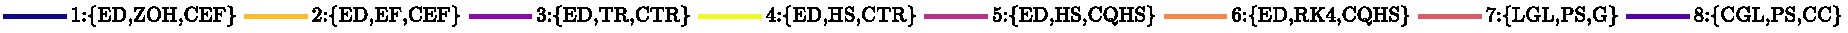
\includegraphics[width=\textwidth]{../ch5/figures/ex1_sens_legend}%

\vspace{1mm}

\begin{subfigure}{0.5\textwidth}
\centering
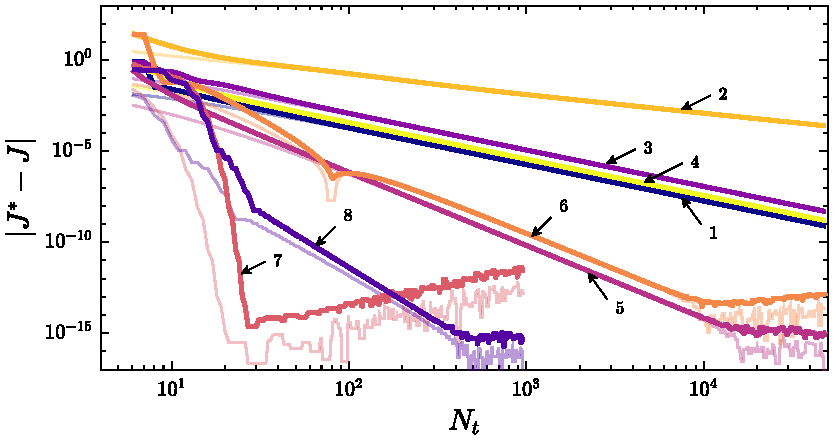
\includegraphics[width=\textwidth]{../ch5/figures/ex1_sens_objective}%
\caption{Objective error.}
\label{fig:ch5:ex1sens:objective}
\end{subfigure}%
\begin{subfigure}{0.5\textwidth}
\centering
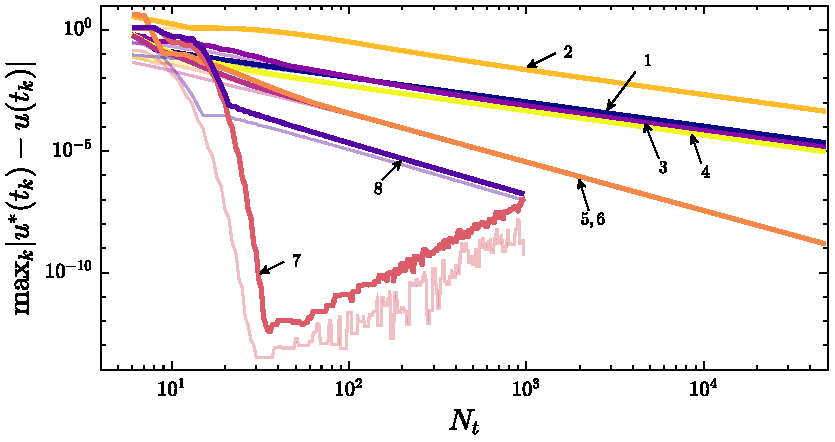
\includegraphics[width=\textwidth]{../ch5/figures/ex1_sens_control}%
\caption{Control error.}
\label{fig:ch5:ex1sens:control}
\end{subfigure}%

\begin{subfigure}{0.5\textwidth}
\centering
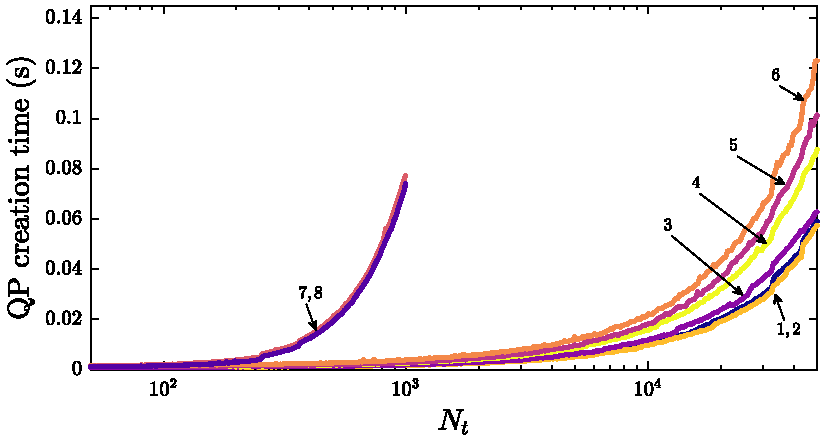
\includegraphics[width=\textwidth]{../ch5/figures/ex1_sens_qp_time}%
\caption{\qp{} creation time vs. $N_t$.}
\label{fig:ch5:ex1sens:qptime}
\end{subfigure}%
\begin{subfigure}{0.5\textwidth}
\centering
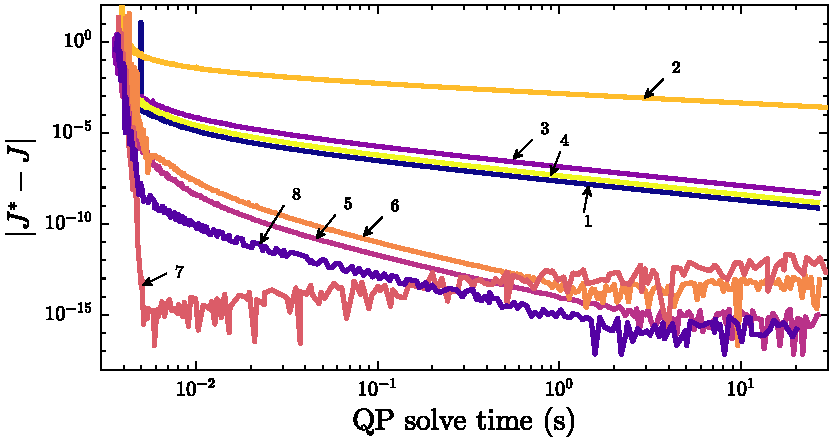
\includegraphics[width=\textwidth]{../ch5/figures/ex1_sens_solve_time}%
\caption{Objective error vs. total \qp{} solve time.}
\label{fig:ch5:ex1sens:solvetime}
\end{subfigure}%

\caption{Numerical results for \nameref{sec:ch5:example1}.}
\label{fig:ch5:ex1sens}
\end{figure}%

% new paragraph (qp creation time)
The time to create the \qp{} vs.~$N_t$ for each scheme is shown in Fig.~\ref{fig:ch5:ex1sens:qptime}.
Here we see two distinct groups: one for the PS-based schemes, and one for the SS-based schemes.
The PS-based schemes take a longer amount of time for a specific $N_t$ because the sparse matrices are much denser (cf. Fig.~\ref{fig:figsparsityAPS} and Fig.~\ref{fig:figsparsityASS}).
The primary cost is the construction of the sparse matrices from the sequences.
The SS-based schemes do vary in their creation time with the schemes, with more matrix calculations and denser defect constraint matrices being slower to create.
Therefore, we observe that (1) is the fastest and (6) is the slowest.
All creation times for this problem are under 0.13~s, even for larger $N_t$.

% new paragraph (qp solve time)
A fairer comparison between the schemes considers the tradeoffs between accuracy and total solve time.
The time to create and solve the \qp{} vs. the error in the objective function is shown in Fig.~\ref{fig:ch5:ex1sens:solvetime}.
The ordering is generally the same as the error plots, and (7) is clearly the preferred scheme for this problem.
Schemes (5) and (6) are slightly more attractive as the computation time for a given error is only slightly slower than the PS-based schemes.